\documentclass[
	a4paper,
	oneside,
	BCOR = 10mm,
	DIV = 12,
	12pt,
	headings = normal,
]{scrartcl}

%%% Length calculations
\usepackage{calc}
%%%

%%% Support for color
\usepackage{xcolor}
\definecolor{lightblue}{HTML}{03A9F4}
\definecolor{red}{HTML}{F44336}
%%%

%%% Including graphics
\usepackage{graphicx}
%%%

%%% Font selection
\usepackage{fontspec}

\setromanfont{STIX Two Text}[
	SmallCapsFeatures = {LetterSpace = 8},
]

\setsansfont{IBM Plex Sans}[
	Scale = MatchUppercase,
]

\setmonofont{IBM Plex Mono}[
	Scale = MatchUppercase,
]
%%%

%%% Math typesetting
\usepackage{amsmath}

\usepackage{unicode-math}
\setmathfont{STIX Two Math}
%%%

%%% List settings
\usepackage{enumitem}
\setlist[enumerate]{
	label*      = {\arabic*.},
	leftmargin  = *,
	labelindent = \parindent,
	topsep      = 1\baselineskip,
	parsep      = 0\baselineskip,
	itemsep     = 1\baselineskip,
}

\setlist[itemize]{
	label*      = {—},
	leftmargin  = *,
	labelindent = \parindent,
	topsep      = 1\baselineskip,
	parsep      = 0\baselineskip,
	itemsep     = 1\baselineskip,
}

\setlist[description]{
	font        = {\rmfamily\upshape\bfseries},
	topsep      = 1\baselineskip,
	parsep      = 0\baselineskip,
	itemsep     = 0\baselineskip,
}

%%%

%%% Structural elements typesetting
\setkomafont{pagenumber}{\rmfamily}
\setkomafont{disposition}{\rmfamily\bfseries}

% Sectioning
\RedeclareSectionCommand[
	beforeskip = -1\baselineskip,
	afterskip  = 1\baselineskip,
	font       = {\normalsize\bfseries\scshape},
]{section}

\RedeclareSectionCommand[
	beforeskip = -1\baselineskip,
	afterskip  = 1\baselineskip,
	font       = {\normalsize\bfseries\itshape},
]{subsection}

\RedeclareSectionCommand[
	beforeskip = -1\baselineskip,
	afterskip  = 1\baselineskip,
	font       = {\normalsize\bfseries},
]{subsubsection}

\RedeclareSectionCommand[
	beforeskip = -1\baselineskip,
	afterskip  = -0.5em,
	font       = {\normalsize\mdseries\scshape\addfontfeatures{Letters = {UppercaseSmallCaps}}},
]{paragraph}
%%%

%%% Typographic enhancements
\usepackage{microtype}
%%%

%%% Language-specific settings
\usepackage{polyglossia}
\setmainlanguage{ukrainian}
\setotherlanguages{english}
%%%

%%% Captions
\usepackage{caption}
\usepackage{subcaption}

%\DeclareCaptionLabelFormat{closing}{#2)}
%\captionsetup[subtable]{labelformat = closing}

%\captionsetup[subfigure]{labelformat = closing}

\captionsetup[table]{
	aboveskip = 0\baselineskip,
	belowskip = 0\baselineskip,
}

\captionsetup[figure]{
	aboveskip = 1\baselineskip,
	belowskip = 0\baselineskip,
}

\captionsetup[subfigure]{
	labelformat = simple,
	labelformat = brace,
}
%%%

%%% Hyphenated ragged typesetting
\usepackage{ragged2e}
%%%

%%% Table typesetting
\usepackage{booktabs}
\usepackage{longtable}

\usepackage{multirow}

\usepackage{array}
\newcolumntype{v}[1]{>{\RaggedRight\arraybackslash\hspace{0pt}}p{#1}}
\newcolumntype{b}[1]{>{\Centering\arraybackslash\hspace{0pt}}p{#1}}
\newcolumntype{n}[1]{>{\RaggedLeft\arraybackslash\hspace{0pt}}p{#1}}
%%%

%%% Drawing
\usepackage{tikz}
\usepackage{tikzscale}
\usetikzlibrary{positioning}
\usetikzlibrary{arrows.meta} % Stealth arrow tips
%%%

%%% SI units typesetting
\usepackage{siunitx}
\sisetup{
	output-decimal-marker = {,},
	exponent-product      = {\cdot},
	inter-unit-product    = \ensuremath{{} \cdot {}},
	per-mode              = symbol,
}
%%%

%%% Bibliography
\usepackage[
	style    = gost-numeric,
	language = auto,
	autolang = other,
	sorting  = none,
]{biblatex}
\addbibresource{y03s01-telecom-homework-01-bibliography.bib}
%%%

%%% Links and hyperreferences
\usepackage{hyperref}
\hypersetup{
	bookmarksnumbered = true,
	colorlinks      = false,
	linkbordercolor = red,
	urlbordercolor  = lightblue,
	pdfborderstyle  = {/S/U/W 1.5},
}
%%%

%%% Length adjustments
% Set baselineskip, default is 14.5 pt
\linespread{1.068966} % ~15.5 pt
\setlength{\emergencystretch}{1em}
\setlength{\parindent}{1.5em}
\newlength{\gridunitwidth}
\setlength{\gridunitwidth}{\textwidth / 12}
%%%

%%% Custom commands
\newcommand{\allcaps}[1]{{\addfontfeatures{LetterSpace = 8, Kerning = Off}#1}}
%%%

\begin{document}

\begin{titlepage}
		\begin{center}
			Міністерство освіти і науки України\\
			Національний авіаційний університет\\
			Навчально-науковий інститут комп'ютерних інформаційних технологій\\
			Кафедра комп'ютеризованих систем управління

			\vspace{\fill}
				Домашнє завдання\\
				з дисципліни «Телекомунікаційні~технології комп'ютерних~мереж»\\
				на тему «Технологія \textenglish{FDDI}»

			\vspace{\fill}

			\begin{flushright}
				Виконав:\\
				студент \allcaps{ННІКІТ}\\
				групи СП-325\\
				Клокун В.\,Д.\\
				Перевірив:\\
				Пушкін Ю.\,О.
			\end{flushright}

			Київ 2018
		\end{center}
	\end{titlepage}

	\section{Короткі відомості}
		\textenglish{FDDI}~(\textenglish{Fiber Distributed Data Interface~— розподілений інтерфейс передачі даних по оптичному волокну})~— це стандарт передачі даних, який визначає локальну мережу з~подвійним кільцем та~методом доступу з~передачею маркера на швидкості~\SI{100}{\mega\bit\per\second}~\cite{cisco-docwiki-fddi}. Стандарт \textenglish{FDDI} був випущений \textenglish{ANSI} в середині 1986~року Американським національним інститутом стандартів~(\textenglish{ANSI}) і~отримав номер \textenglish{ANSI X3T9.5}~\cite{wiki-uk-fddi}.
		
		\textenglish{FDDI} часто використовується як високошвидкісна основна технологія завдяки підтримці високої пропускної здатності та більш дальніх відстаней порівняно з технологіями на основі мідних середовищ передачі. Варто зазначити, що існує схожа специфікація з мідною середою передачі~— \textenglish{Copper Distributed Data Interface (CDDI)}.

		Технологія \textenglish{FDDI} використовує подвійну кільцеву архітектуру~(рис.~\ref{fig:dual-ring-topology}), в кожному кільці якої трафік рухається в протилежних напрямках. Таке подвійне кільце складається з основного та додаткового кільця. Під час нормальної роботи основне кільце використовується для передачі даних, а побічне знаходиться у стані простою. Основною ціллю використання двох кілець є надання більшої надійності.

		\begin{figure}[!htbp]
			\centering
			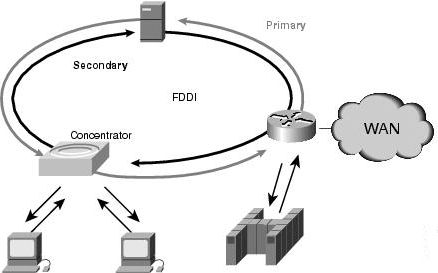
\includegraphics[height = 8\baselineskip]{./assets/y03s01-telecom-homework-01-p01-fddi-counter-rotating.jpg}
			\caption{Топологія подвійного кільця в~\textenglish{FDDI}}
			\label{fig:dual-ring-topology}
		\end{figure}

	\section{Середа передачі даних~\textenglish{FDDI}}
		Технологія \textenglish{FDDI} використовує оптичне волокно як основну середу передачі даних. Використання оптичного волокна має декілька переваг перед мідними кабелями, а саме безпека, стійкість та швидкодія покращуються, оскільки оптичне волокно не випромінює електричні сигнали. Дані, які передаються у середовищі передачі, в якому використовуються електричні сигнали, можуть бути перехоплені, тобто існує ризик неавторизованого доступу до передаваних даних. Крім того, оптичне волокно стійке до радіочастотної та електромагнітної інтерференції, а також має більшу пропускну здатність порівняно з міддю. Також, технологія~\textenglish{FDDI} дозволяє передавати дані між станціями на відстані~\SI{2}{\kilo\metre}, використовуючи багатомодове волокно, та на більші відстані з одномодовим.

		Технологія~\textenglish{FDDI} визначає 2 типи оптичного волокна: одномодове та багатомодове~(рис.~\ref{fig:single-and-multimode-fibre}). Мода — це пучок світла, який падає у світловод оптичного волокна під певним кутом. При використанні багатомодового волокна у якості світлогенеруючих пристроїв зазвичай використовують світлодіоди, коли з одномодовим використовують лазери.

		У багатомодовому волокні розповсюджується декілька мод світла. Оскільки такі світлові моди потрапляють у оптичне волокно під різними кутами, вони досягнуть кінця у різний час. Ця характеристика називається модовою дисперсією. Модова дисперсія обмежує пропускну здатність та відстань, на яку можна здійснити передачу за допомогою багатомодових волокон, тому вони зазвичай використовуються для встановлення зв'язку в межах будівель або відносно невеликих середовищ.

		В одномодовому волокні розповсюджується лише одна світлова мода. Оскільки використовується лише одна мода, модова дисперсія відсутня, тому одномодове волокно здатне надавати значно більшу продуктивність на значно більших відстанях, завдяки чому воно зазвичай використовується для організації зв'язку між більш віддаленими будівлями та областями.

		\begin{figure}[!htbp]
			\centering
			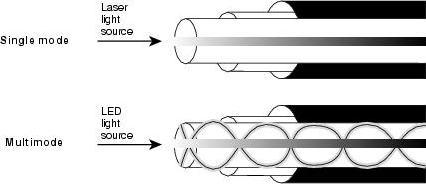
\includegraphics[height = 8\baselineskip]{./assets/y03s01-telecom-homework-01-p02-optical-fibres.jpg}
			\caption{Одномодове та багатомодове оптичне волокно}
			\label{fig:single-and-multimode-fibre}
		\end{figure}

	\section{Специфікація технології~\textenglish{FDDI}}
		Технологія~\textenglish{FDDI} визначає фізичну та канальні рівні моделі~\textenglish{OSI}. Технологія~\textenglish{FDDI} насправді не є однією специфікацією, а збіркою чотирьох окремих, кожна з яких визначає певну функцією. Використання цих специфікацій разом дає змогу надавати високошвидкісну взаємодію між протоколами вищих рівней на кшталт~\textenglish{TCP/IP, IPX} та середовищами передачі на кшталт волоконно-оптичних кабелів.

		До складу технології~\textenglish{FDDI} входять 4 специфікації~(рис.~\ref{fig:fddi-osi-mapping}):
		\begin{enumerate}
			\item \textenglish{Media Access Control} (\textenglish{MAC}, Управління доступом до носія)~— визначає спосіб доступу до носія, включаючи формат пакета, обробку маркера, адресацію, алгоритм перевірки надлишковості циклу (\textenglish{CRC}) та механізми корекції помилок.
			\item \textenglish{Physical Layer Protocol} (\textenglish{PHY}, Протокол фізичного рівня)~— визначає процедури кодування та декодування інформації, вимоги до синхронізації, формування кадрів та інше.
			\item \textenglish{Physical-Medium Dependent} (\textenglish{PMD}, Середовищезалежне)~— визначає характеристики середовища передачі, включаючи волоконно-оптичні лінії зв'язку, рівні потужності, коефіцієнт бітових помилок, оптичні компоненти та конектори.
			\item \textenglish{Station Management} (\textenglish{SMT}, Управління станціями)~— визначає конфігурацію станцій~\textenglish{FDDI}, конфігурацію кільцевої мережі та особливості управління ціжю мережею, включаючи вставку та виключення станцій, ініціалізацію, ізоляцію та усунення несправностей, створення графіка та сбір статистики.
		\end{enumerate}

		\begin{figure}[!htbp]
			\centering
			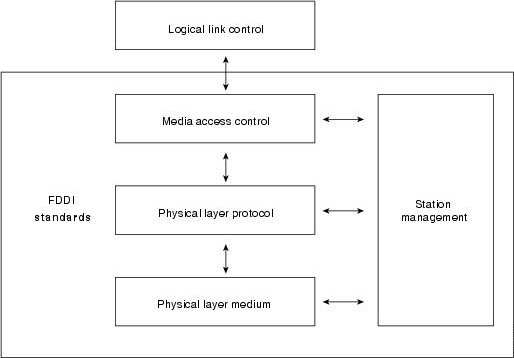
\includegraphics[height = 10\baselineskip]{./assets/y03s01-telecom-homework-01-p03-fddi-to-osi-map.jpg}
			\caption{Відповідність між специфікаціями~\textenglish{FDDI} та моделлю~\textenglish{OSI}}
			\label{fig:fddi-osi-mapping}
		\end{figure}

	\section{Типи підключення станцій~\textenglish{FDDI}}
		Однією з визначних характеристик технології~\textenglish{FDDI} є наявність можливості підключити \textenglish{FDDI}-сумісні пристрої декількома способам.и. Технологія~\textenglish{FDDI} визначає 4 типи пристроїв:
		\begin{enumerate}
			\item Станція з одним підключенням (\textenglish{Single-attachment station, SAS}).
			\item Станція з подвійним підключенням (\textenglish{Dual-attachment station, DAS)}.
			\item Концентратор з одним підключенням (\textenglish{Single-attachment concentrator, SAC}).
			\item Концентратор з подвійним підключенням (\textenglish{Dual-attachment concentrator, DAC}).
		\end{enumerate}

		Станції з одним підключенням підключаються лише до одного кільця (основного) за допомогою концентратора. Однією з основних переваг підключення пристроїв з одним підключенням є те, що вимкнення або відключення пристрою ніяк не вплине на кільце~\textenglish{FDDI}.

		Станції з подвійним підключенням мають два порти: A і~B~(рис.~\ref{fig:das-ports}). За допомогою цих портів станція з подвійним підключенням підключається до обох кілець~\textenglish{FDDI}, тобто кожен порт встановлює зв'язок між основним та додатковим кільцем. Вимкнення або відключення пристроїв з подвійним підключенням матиме вплив на кільце~\textenglish{FDDI}.

		\begin{figure}[!htbp]
			\centering
			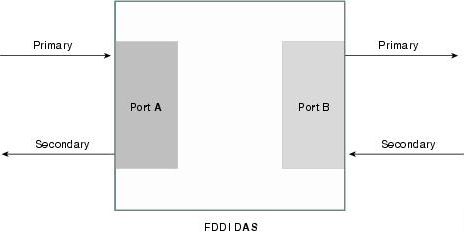
\includegraphics[height = 10\baselineskip]{./assets/y03s01-telecom-homework-01-p04-das-ports.jpg}
			\caption{Порти станції з подвійним підключенням}
			\label{fig:das-ports}
		\end{figure}

		Концентратор з подвійним підключенням підключається до основного та додаткового кільця~(рис.~\ref{fig:das-attachment}) та дозволяє впевнитись, що збій або відключення будь-якої станції з одним підключенням не викличе повну відмову кільця~\textenglish{FDDI}. Це особливо зручно, коли до кільця підключаються пристрої, які часто вмикаються та вимикаються, наприклад, персональні комп'ютери.

		\begin{figure}[!htbp]
			\centering
			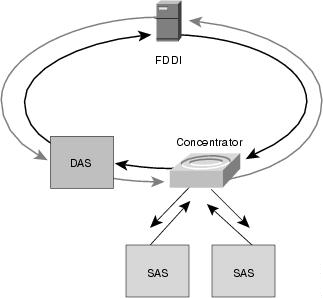
\includegraphics[height = 8\baselineskip]{./assets/y03s01-telecom-homework-01-p05-das-attachment.jpg}
			\caption{Підключення концентратора з подвійним підключенням до кільця~\textenglish{FDDI}}
			\label{fig:das-attachment}
		\end{figure}

	\section{Стійкість до відмов}
		Технологія~\textenglish{FDDI} надає декілька можливостей для організації стійкості до відмов, а саме: подвійне кільце, оптичні обхідні перемикачі та підтримку двопортового~(\textenglish{dual-homing}) підключення.

		\subsection{Подвійне кільце}
			Використання архітектури з подвійним кільцем є основною можливістю технології~\textenglish{FDDI} із забезпечення стійкості до відмов. Якщо станція у подвійному кільці дає збій або пошкоджується з'єднувальний кабель, подвійне кільце автоматично згортається в одне, тобто топологія з подвійним кільцем перетворюється в звичайну кільцеву топологію~(рис.~\ref{fig:fddi-fault-tolerance-dual-ring}). Дані продовжують передаватись кільцем~\textenglish{FDDI} без втрат продуктивності навіть у режимі згортання.

			\begin{figure}[!htbp]
				\centering
				\begin{subfigure}[t]{0.5\textwidth}
					\centering
					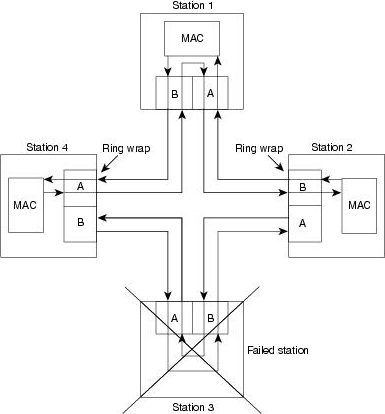
\includegraphics[height = 10\baselineskip]{./assets/y03s01-telecom-homework-01-p06a-station-failure.jpg}
					\caption{}
					\label{subfig:fddi-fault-tolerance-dual-ring-station-failure}
				\end{subfigure}%
				\begin{subfigure}[t]{0.5\textwidth}
					\centering
					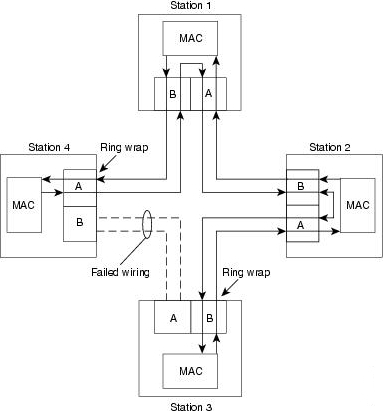
\includegraphics[height = 10\baselineskip]{./assets/y03s01-telecom-homework-01-p06b-cable-failure.jpg}
					\caption{}
					\label{subfig:fddi-fault-tolerance-dual-ring-cable-failure}
				\end{subfigure}%
				\caption{Стійкість подвійного кільця до відмов: \subref{subfig:fddi-fault-tolerance-dual-ring-station-failure}~— у разі виходу станції з ладу, \subref{subfig:fddi-fault-tolerance-dual-ring-cable-failure}~— у разі пошкодження кабеля}
				\label{fig:fddi-fault-tolerance-dual-ring}
			\end{figure}

			Коли трапляється збій однієї станції~(рис.~\ref{subfig:fddi-fault-tolerance-dual-ring-station-failure}), пристрої з обох боків непрацюючої станції згортаються, формуючи єдине кільце~\cite{olifer-networks-4th-ed}. Мережа продовжує працювати для залишившихся станцій на кільці. У випадку пошкодження кабелю~(рис.~\ref{subfig:fddi-fault-tolerance-dual-ring-cable-failure}) згортаються пристрої з обох боків місця пошкодження кабелю, мережа продовжує роботу для усіх станцій.

			Варто зазначити, що~\textenglish{FDDI} забезпечує стійкість до одного збою. У випадку двох або більше збоїв кільце~\textenglish{FDDI} ділиться на два або більше незалежні кільця, які не можуть зв'язатись одне з одним.

		\subsection{Оптичний обхідний перемикач}
			Оптичний обхідний перемикач забезпечує безперервну роботу в режимі подвійного кільця, якщо певний пристрій, підключений до нього, виходить з ладу~(рис.~\ref{fig:optical-bypass-switch}). Такий підхід використовується для запобігання сегментації кільця та усунення з кільця станцій, що вийшли з ладу. У режимі нормальної роботи оптичний обхідний перемикач виконує цю функцію за допомогою оптичних дзеркал, які передають світло з кільця напряму до пристрою з подвійним підключенням. Якщо пристрій з подвійним підключенням вимикається або виходить з ладу, перемикач за допомогою внутрішніх дзеркал передає світло через себе і таким чином підтримує цілісність кільця.

			\begin{figure}[!htbp]
				\centering
				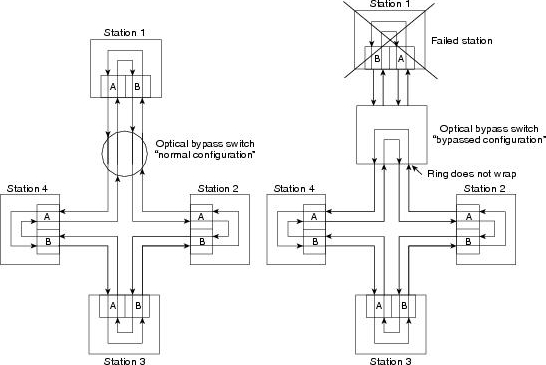
\includegraphics[height = 10\baselineskip]{./assets/y03s01-telecom-homework-01-p07-optical-bypass-switch.jpg}
				\caption{Оптичний обхідний перемикач підтримує роботу мережі}
				\label{fig:optical-bypass-switch}
			\end{figure}

			Перевагою такої можливості є те, що кільце не згорнеться у випадку збою пристрою.

		\subsection{Двопортове підключення}
			Для забезпечення додаткової надлишковості та гарантування нормальної роботи критично важливих пристроїв, наприклад, маршрутизаторів або мейнфреймів, можна використовувати двопортове підключення, при якому важливий пристрій підключається до двох концентраторів~(рис.~\ref{fig:dual-homing}).

			\begin{figure}
				\centering
				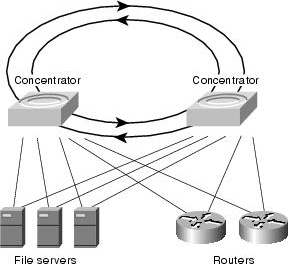
\includegraphics[height = 10\baselineskip]{./assets/y03s01-telecom-homework-01-p08-dual-homing.jpg}
				\caption{Дворазове підключення}
				\label{fig:dual-homing}
			\end{figure}

			Одне з'єднання концентратора називається активним, а інше~— пасивним. Пасивне з'єднання залишається у резервному режимі до тих пір, поки основне з'єднання або концентратор, до якого воно підключене, не виходять з ладу. У випадку виходу з ладу автоматично активується пасивне з'єднання.

	\section{Формат кадрів~\textenglish{FDDI}}
		Формат кадрів~\textenglish{FDDI} схожий на формат кадрів~\textenglish{Token Ring}, їх розмір може досягати~\SI{4500}{\byte}.

		\begin{figure}[!htbp]
			\centering
			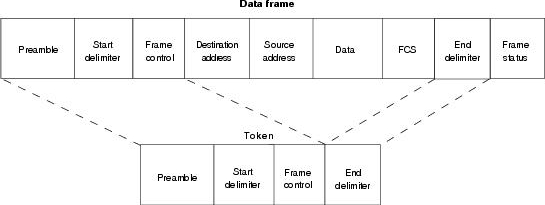
\includegraphics[height = 10\baselineskip]{./assets/y03s01-telecom-homework-01-p09-fddi-frame-format.jpg}
			\caption{Формат кадру~\textenglish{FDDI}}
			\label{fig:fddi-frame-format}
		\end{figure}

		Кадр~\textenglish{FDDI} має такі поля~(рис.~\ref{fig:fddi-frame-format}):
		\begin{enumerate}
			\item \textenglish{Preamble} (преамбула)~— містить спеціальну послідовність даних, яка готує кожну станцію для майбутнього кадру.
			\item \textenglish{Start delimiter} (початковий розділяючий знак)~— позначає початок кадру за допомогою сигнальної послідовності даних, яка відрізняє його від іншої частини кадру.
			\item \textenglish{Frame control} (управляюча інформація кадру)~— позначає розмір адресних полів та тип даних, які містить кадр~(синхронні або асинхронні), а також іншу управляючу інформацію.
			\item \textenglish{Destination address} (адреса призначення)~— містить адресу призначення одиночної~(\textenglish{unicast}), групової~(\textenglish{multicast}) та широкомовної передачі~(\textenglish{broadcast}).
			\item \textenglish{Source address} (адреса джерела)~— містить дані, що ідентифікують станцію, яка надіслала кадр. Як і у~\textenglish{Ethernet} та~\textenglish{Token Ring}, довжина адреси у~\textenglish{FDDI}~— \SI{6}{\byte}.
			\item \textenglish{Data} (дані)~— містить дані, призначені для протоколу вищого рівня, або управляючу інформацію.
			\item \textenglish{Frame check sequence} (послідовність перевірки кадру)~— містить значення циклічного надлишкового коду~(\textenglish{CRC}), яке залежить від вмісту кадру та передається станцією-джерелом передачі. Отримувач заново обчислює значення, щоб визначити, чи був кадр пошкоджений у передачі. Якщо кадр був пошкоджений, він відкидається.
			\item \textenglish{End delimiter} (кінцевий розділяючий знак)~— позначає кінець кадру.
			\item \textenglish{Frame status} (статус кадру)~— дозволяє станції-джерелу визначити, чи сталась помилка, та визначає, чи успішно приймаюча станція отримала та розпізнала кадр.
		\end{enumerate}

	\section{Висновок}
		Розподілений інтерфейс передачі даних по оптичному волокну~— це перша технологія локальних мереж, в якій вперше в якості середовища передачі даних став використовуватись волоконно-оптичний кабель. Ця технологія дозволяє передавати дані на швидкості~\SI{100}{\mega\bit\per\second} в подвійному кільці довжиною до~\SI{200}{\kilo\metre} і організує доступ до носія за допомогою передачі маркера.

		Ця технологія є суттєвим покращенням технології~\textenglish{Token Ring} в областях швидкості і дальності передачі завдяки використанню волоконно-оптичного кабеля, та стійкості до відмов завдяки використанню подвійного кільця.

	{
	% \raggedright
	\printbibliography
	}

\end{document}
